%draft 选项可以使插入的图形只显示外框,以加快预览速度。
%fleqn 让公式左对齐。
\documentclass[12pt,a4paper,openany,twoside]{book}
\usepackage{amsmath}  %数学公式
\usepackage{amssymb} %数学符号
\usepackage{mathrsfs}   % 不同于\mathcal or \mathfrak 之类的英文花体字体
\usepackage{float}
\usepackage{units}
\usepackage{multirow}
\usepackage{graphicx}
\usepackage{setspace}
\usepackage{xCJKnumb} %使用汉字 章
%\usepackage{subfigure}  % 并列的图形
\usepackage{setspace}       % 定制表格和图形的多行标题行距
\usepackage{supertabular}   % 使用跨页表格的宏包
\usepackage{longtable}       %长表格,可以跨页
\usepackage{tabularx}       %可以换行的表格
\usepackage{booktabs}       %\toprule、\midrule 和 \bottomrule,可分别对表格顶部、中部和底部使用不同粗细的水平线
\usepackage{array}          %固定列宽可以使用array宏包的p{2cm}系列命令,需要指定水平对齐方式,可以使用下面的形式: >{\centering}p{2cm}
\usepackage{makeidx}        % 生成索引
\usepackage{listings}       %支持编程语言源代码的宏包
%\usepackage{xcolor}   

%===图片处理宏包=============================
%\usepackage{subfigure}  % 并列的图形
%\usepackage{color}      % 支持彩色

% 版面控制宏包,定义规定的版面尺寸============
%\usepackage[%paperwidth=18.4cm, paperheight= 26cm,
%            body={14.6true cm,22.0true cm},
%            twosideshift=0 pt,
%            %headheight=1.0true cm
%            ]{geometry}
\usepackage[top=2cm,bottom=2.5cm,left=2.8cm,right=2.8cm,includehead,includefoot%
            ]{geometry}  


\usepackage[perpage,symbol]{footmisc}% 脚注控制
\usepackage{fancyhdr} %页眉页脚
\usepackage[square,super,comma,sort,compress]{natbib} %文献格式
\usepackage{titletoc}
\usepackage{titlesec}
\usepackage[dvipsnames,svgnames,x11names]{xcolor} %彩色工具
\usepackage[CJKbookmarks=true]{hyperref}
% 定理类环境宏包,其中 amsmath 选项用来兼容 AMS LaTeX 的宏包
\usepackage[amsmath,thmmarks]{ntheorem}

%\usepackage{subeqnarray} %多个子方程(1-1a)(1-1b)
%\iffalse 以下是一个例子
%\begin{subeqnarray}
%\label{eqw} \slabel{eq0}
% x & = & a \times b \\
%\slabel{eq1}
% & = & z + t\\
%\slabel{eq2}
% & = & z + t
%\end{subeqnarray}
%\fi

%首行缩进
%\parindent=2em
\makeatletter
\let\@afterindentfalse\@afterindenttrue
\@afterindenttrue
\makeatother
\setlength{\parindent}{2em}
%% 定义正文字体
\usepackage{fontspec}
\usepackage[BoldFont,CJKnumber]{xeCJK}
\setmainfont{Times New Roman} % 英文字体 
\setmonofont{Consolas}
%\setmonofont{Courier New}
\setCJKmainfont{Adobe 宋体 Std} %正文字体  适用于OS X,其他OS可换为SimSun等
\setCJKfamilyfont{song}{Adobe 宋体 Std}
\setCJKfamilyfont{hei}{Adobe 黑体 Std}
\setCJKfamilyfont{kai}{Adobe 楷体 Std}
\newcommand\song{\CJKfamily{song}}
\newcommand\hei{\CJKfamily{hei}}
\newcommand\kai{\CJKfamily{kai}}

\renewcommand{\baselinestretch}{1.5} %正文行距
\usepackage{xunicode}% provides unicode character macros
\usepackage{xltxtra} % provides some fixes/extras
\usepackage{url}




% 重定义字号命令
\newcommand{\xiaochu}{\fontsize{30pt}{40pt}\selectfont}    % 小初, 1.5倍行距
\newcommand{\yihao}{\fontsize{26pt}{36pt}\selectfont}    % 一号, 1.4倍行距
\newcommand{\erhao}{\fontsize{22pt}{28pt}\selectfont}    % 二号, 1.25倍行距
\newcommand{\xiaoer}{\fontsize{18pt}{18pt}\selectfont}    % 小二, 单倍行距
\newcommand{\sanhao}{\fontsize{16pt}{24pt}\selectfont}    % 三号, 1.5倍行距
\newcommand{\xiaosan}{\fontsize{15pt}{22pt}\selectfont}    % 小三, 1.5倍行距
\newcommand{\sihao}{\fontsize{14pt}{21pt}\selectfont}    % 四号, 1.5倍行距
\newcommand{\banxiaosi}{\fontsize{13pt}{19.5pt}\selectfont}    % 半小四, 1.5倍行距
\newcommand{\xiaosi}{\fontsize{12pt}{18pt}\selectfont}    % 小四, 1.5倍行距
\newcommand{\dawuhao}{\fontsize{11pt}{11pt}\selectfont}    % 大五号, 单倍行距
\newcommand{\wuhao}{\fontsize{10.5pt}{10.5pt}\selectfont}    % 五号, 单倍行距
\newcommand{\xiaowu}{\fontsize{9pt}{9pt}\selectfont}    % 小五号, 单倍行距





%页眉页脚
\pagestyle{fancy}
\renewcommand{\sectionmark}[1]{\markright{\small\thesection\quad #1}{}}
\renewcommand{\chaptermark}[1]{\markboth{\small 第\,\xCJKnumber{\thechapter}\,章\quad #1}{}}
\fancyhf{}   
\fancyhead[CE]{\song \wuhao\rightmark}
\fancyhead[CO]{\song \wuhao \leftmark}
\fancyfoot[CO,CE]{\wuhao{\thepage}}%


%%% 
%%% %%% Clear Header %%%%%%%%%%%%%%%%%%%%%%%%%%%%%%%%%%%%%%%%%%%%%%%%%%%
% Clear Header Style on the Last Empty Odd pages
\makeatletter
\def\cleardoublepage{\clearpage\if@twoside \ifodd\c@page\else%
    \hbox{}%
    \thispagestyle{empty}%              % Empty header styles
    \newpage%
    \if@twocolumn\hbox{}\newpage\fi\fi\fi}




%% 正文标题格式
\titleformat{\chapter}[hang]{ \centering\xiaosan\hei\bfseries}{第\,\xCJKnumber{\thechapter}\,章}{1em}{} %章:小三黑体加粗并居中
\titleformat{\section}[hang]{\hei\sihao\bfseries}{\thesection{}}{1em}{} %节:四号黑体加粗
\titleformat{\subsection}[hang]{\bfseries\hei\xiaosi}{\thesubsection}{0.5em}{} %目:小四黑体加粗
\titleformat{\subsubsection}[hang]{\bfseries\hei\xiaosi}{\thesubsubsection}{0.5em}{} %子目:小四黑体加粗
%标题间距
\titlespacing{\chapter}{0bp}{-30bp}{12bp}
\titlespacing{\section}{0bp}{0bp}{12bp}
\titlespacing{\subsection}{0bp}{12bp}{0bp}
\titlespacing{\subsubsection}{0bp}{12bp}{0bp}
   
% 图表定义
\renewcommand{\figurename}{\bfseries \song \xiaosi 图}
\numberwithin{figure}{chapter}
\renewcommand{\tablename}{\bfseries \song \xiaoso  表}
\numberwithin{table}{chapter}
\renewcommand{\thefigure}{\thechapter.\arabic{figure}}
\renewcommand{\thetable}{\thechapter.\arabic{table}}
%\renewcommand{\lstlistingname}{\bfseries \song \xiaowu 算法}
%\def\thelstlisting{\thesection.\arabic{lstlisting}}



%公式按章编号
\numberwithin{equation}{chapter}
\renewcommand{\theequation}{\thechapter-\arabic{equation}} 



%%%%%%%%%%%%%%%%%%%%%%%%%%%%%%%%%%%%%%%%%%%%%%%%%%%%%%%%%%%%%%%%%%%%%%
% 封面、摘要、版权、致谢格式定义
%%%%%%%%%%%%%%%%%%%%%%%%%%%%%%%%%%%%%%%%%%%%%%%%%%%%%%%%%%%%%%%%%%%%%%
\def\ctitle#1{\def\@ctitle{#1}}\def\@ctitle{}
\def\cdegree#1{\def\@cdegree{#1}}\def\@cdegree{}
\def\caffil#1{\def\@caffil{#1}}\def\@caffil{}
\def\csubject#1{\def\@csubject{#1}}\def\@csubject{}
\def\cauthor#1{\def\@cauthor{#1}}\def\@cauthor{}
\def\cnumber#1{\def\@cnumber{#1}}\def\@cnumber{}
\def\csubsub#1{\def\@csubsub{#1}}\def\@csubsub{}
\def\csupervisor#1{\def\@csupervisor{#1}}\def\@csupervisor{}
\def\cdate#1{\def\@cdate{#1}}\def\@cdate{}
\def\ddate#1{\def\@ddate{#1}}\def\@ddate{}
\long\def\cabstract#1{\long\def\@cabstract{#1}}\long\def\@cabstract{}
\def\ckeywords#1{\def\@ckeywords{#1}}\def\@ckeywords{}

\def\etitle#1{\def\@etitle{#1}}\def\@etitle{}
\long\def\eabstract#1{\long\def\@eabstract{#1}}\long\def\@eabstract{}
\def\ekeywords#1{\def\@ekeywords{#1}}\def\@ekeywords{}




%中文封面%%%%%%%%%%%%%%%%%%%%%%%%%%%%%%%%%%%%%%%%%%%%%%%%%%%
\def\makecover{
    \begin{titlepage}
    \newpage
    \thispagestyle{empty}

    \begin{minipage}[b][0cm][b]{9cm}
    \begin{flushleft}
    \song \xiaosi \bfseries {学校编码:10384}\\
    \song \xiaosi \bfseries {学号:\@cnumber}
    \end{flushleft}

    \end{minipage} \hfill

    \parbox[r][0cm][r]{13.6cm}{
    \begin{flushright}
    \song \xiaosi \bfseries {分类号\underline{~~~~~~~~~~~~~~}密级\underline{~~~~~~~~~~~~}}\\
    \song \xiaosi \bfseries {UDC\underline{~~~~~~~~~~~~~~}}
    \end{flushright}}

    \begin{center}

    \begin{figure}[htb!]
        \centering
        
\includegraphics[width=6.2cm,bb=0 0 200 62]{figure/xmulogo.jpg}
    \end{figure}

    \parbox[t][1cm][c]{\textwidth}{\xiaoer
    \begin{center} {
    \song  \@cdegree ~~~~学~~~~位~~~~论~~~~文}\end{center} }

    \parbox[t][5cm][c]{\textwidth}{
    \begin{center}{\erhao \hei \bfseries \@ctitle }\end{center}
    \begin{center}{\sanhao \bfseries \@etitle }\end{center}}

    \parbox[t][1cm][c]{\textwidth}{\xiaoer\kai
    \begin{center} {\@cauthor}
    \end{center} }

    \parbox[t][6.5cm][c]{\textwidth}{ {\sihao\kai
    \begin{center}
    \begin{tabular}{cc@{\extracolsep{1em}}l}
    ~ & 指导教师姓名:& \@csupervisor \\
    ~ & 专~~~业~~~名~~~称:& \@csubject \\
    ~ & 论文提交日期:& \@ddate\\
    ~ & 论文答辩时间:& \@ddate\\
    ~ & 学位授予日期:& \@ddate\\
    \end{tabular}
    \end{center} } }

    \parbox[t][3.3cm][r]{\textwidth}{
    \begin{flushright}
    \song \sihao  {答辩委员会主席:\underline{~~~~~~~~~~~~~~~~~~~~}~~~~~~~~~~~~}\\
    \song \sihao  {评~~~~~~~~阅~~~~~~~~人:\underline{~~~~~~~~~~~~~~~~~~~~}~~~~~~~~~~~~}\\
    \end{flushright}}

    \parbox[b][1.2cm][b]{\textwidth}{
    \begin{center} {\sihao \song \@cdate~年~~~~~~~~月} \end{center} }
    \end{center}

    % 封二 空白页
    \cleardoublepage
    \end{titlepage}
}

%%声明
\long\def\statement{
    \newpage
    \thispagestyle{empty}
    %\defaultfont

    \begin{center}
    \hspace{2em}
    \parbox[t][2cm][t]{\textwidth}{ {\xiaoer \hei \centerline {\textbf{厦门大学学位论文原创性声明}}}}
    \parbox[t][9cm][c]{0.96\textwidth}{ \song \sihao
    \hspace{2em}本人呈交的学位论文是本人在导师指导下,独立完成的研究成果。
    本人在论文写作中参考其他个人或集体已经发表的研究成果,
    均在文中以适当方式明确标明,并符合法律规范和《厦门大学研究生学术活动规范(试行)》。

    \hspace{2em}另外,该学位论文为(\hspace{12em})课题(组)的研究成果,
    获得(\hspace{8em})课题(组)经费或实验室的资助,在
    (\hspace{7em})实验室完成。(请在以上括号内填写课题或课题组负责人或实验室名称,未有此项声明内容的,可以不作特别声明。)
}
    \end{center}

    \parbox[t][4cm][b]{\textwidth}{
    \begin{flushright}
    \song \xiaosi 声明人(签名):~~~~~~~~~~~~~~~~~~~~~~~~~~~~~~~~ \\
    \song \xiaosi 年~~~~~~~~月~~~~~~~~日~~~~~~~~~~~~~~~~
    \end{flushright}}
    \cleardoublepage
}

\def\copyright{
    \newpage
    \thispagestyle{empty}
    %\defaultfont
    \begin{center}
    \parbox[t][2cm][t]{\textwidth}{ {\xiaoer \hei \centerline {\textbf{厦门大学学位论文著作权使用声明}} } }
    \parbox[t][15cm][c]{0.98\textwidth}{ \song \sihao
    \hspace{2em}本人同意厦门大学根据《中华人民共和国学位条例暂行实施办法》等规定保留和使用此学位论文,
    并向主管部门或其指定机构送交学位论文(包括纸质版和电子版),
    允许学位论文进入厦门大学图书馆及其数据库被查阅、借阅。
    本人同意厦门大学将学位论文加入全国博士、硕士学位论文共建单位数据库进行检索,
    将学位论文的标题和摘要汇编出版,采用影印、缩印或者其它方式合理复制学位论文。\\
      本学位论文属于:\\
      (\hspace{3em})1.经厦门大学保密委员会审查核定的保密学位论文,
                 于  年  月  日解密,解密后适用上述授权。\\
      (\hspace{3em})2.不保密,适用上述授权。\\
      (请在以上相应括号内打“√”或填上相应内容。
        保密学位论文应是已经厦门大学保密委员会审定过的学位论文,
        未经厦门大学保密委员会审定的学位论文均为公开学位论文。此声明栏不填写的,默认为公开学位论文,均适用上述授权。)
    }
    \end{center}

    \parbox[t][4cm][c]{\textwidth}{\song \xiaosan
    \begin{flushright}
    \song \xiaosi 声明人(签名):~~~~~~~~~~~~~~~~~~~~~~~~~~~~~~~~ \\
    \song \xiaosi 年~~~~~~~~月~~~~~~~~日~~~~~~~~~~~~~~~~
    \end{flushright}
    }

    \cleardoublepage
}



%% 中文摘要和关键词
\newenvironment{cnabstract}[1][]{%
        \thispagestyle{plain}%
    \fancyfoot{}%
    \def\XMU@keywords{#1}%
        \vspace*{10bp}%
        \begin{center}%
        {\hei\xiaoer 摘~~~~~要}%
        \end{center}
        \vspace{12bp}%
    \par%
}{%
    \par%
    \vspace{12bp}%
    \noindent%
    {\hei\xiaosi 关键词:}\quad{\XMU@keywords}%
    %\let\XMU@keywords=\relax%
    \clearpage%
    %\setcounter{page}{1}%
    \cleardoublepage
}


%% 英文摘要和关键词
\newenvironment{enabstract}[1]{%
        \thispagestyle{plain}%
    \fancyfoot{}%
    \def\XMU@keywords{#1}%
        \vspace*{10bp}%
        \begin{center}%
        {\bfseries\xiaoer Abstract}%
        \end{center}
        \vspace{12bp}%
    \par%
}{%
    \par%
    \vspace{12bp}%
    \noindent%
    {\bfseries\xiaosi Key Words:}\quad{\XMU@keywords}%
    %\let\XMU@keywords=\relax%
    \clearpage%
    %\setcounter{page}{0}%
    \cleardoublepage
}



%%目录设置
\renewcommand\contentsname{\hei \xiaosan 目~~~~~录}
\setcounter{secnumdepth}{4} \setcounter{tocdepth}{2}

\titlecontents{chapter}[3.8em]{\hspace{-3.8em}\hei \sihao \bfseries}{第~\xCJKnumber{\thecontentslabel}~章~~}{}{\titlerule*[4pt]{.}\contentspage}

%修正章节数字在目录的距离
\dottedcontents{section}[40pt]{}{22pt}{0.3pc}
\dottedcontents{subsection}[62pt]{}{32pt}{0.3pc}

%重新定义BiChapter命令,可实现标题手动换行,但不影响目录
\def\BiChapter{\relax\@ifnextchar [{\@BiChapter}{\@@BiChapter}}
\def\@BiChapter[#1]#2#3{\chapter[#1]{#2}
    \addcontentsline{toe}{chapter}{\hei \bfseries \sihao Chapter \thechapter\hspace{0.5em} #3}}
\def\@@BiChapter#1#2{\chapter{#1}
    \addcontentsline{toe}{chapter}{\hei \bfseries \sihao Chapter \thechapter\hspace{0.5em}{\boldmath #2}}}
%目录格式
\newcommand{\BiSection}[2]
{   \section{\hei \xiaosi \bfseries #1}%中文
    \addcontentsline{toe}{section}{\hei \xiaosi \bfseries \protect\numberline{\csname thesection\endcsname}#2}%英文
    
}

\newcommand{\BiSubsection}[2]
{    \subsection{\song \xiaosi #1}
    \addcontentsline{toe}{subsection}{\song \xiaosi \protect\numberline{\csname thesubsection\endcsname}#2}
}

\newcommand{\BiSubsubsection}[2]
{    \subsubsection{#1}
    \addcontentsline{toe}{subsubsection}{\protect\numberline{\csname thesubsubsection\endcsname}#2}
}


%%%%%%%%%%%%%%%%%%%%%%%%%%%%%%%%%%%%%%%%%%%%%%%%%%%%%%%%%%%%%%%%%%%%%%%%%%%%%%%%%%%%%%%%%%%%%%%%%%%%%%%%%%%%%%%%%%%%%%%%%%%%%%
% 英文目录格式
\def\@dotsep{0.75}           % 定义英文目录的点间距
\setlength\leftmargini {0pt}
\setlength\leftmarginii {0pt}
\setlength\leftmarginiii {0pt}
\setlength\leftmarginiv {0pt}
\setlength\leftmarginv {0pt}
\setlength\leftmarginvi {0pt}

\def\engcontentsname{\bfseries \xiaosan Contents}
\newcommand\tableofengcontents{
   \pdfbookmark[0]{Contents}{econtent}
     \@restonecolfalse
   \chapter*{\engcontentsname  %chapter*上移一行,避免在toc中出现。
       \@mkboth{%
          \engcontentsname}{\engcontentsname}}
   \@starttoc{toe}%
   \if@restonecol\twocolumn\fi
   }

%%暂时没有使用
\newcommand{\BiAppendixChapter}[2] % 该附录命令适用于发表文章,简历等
{\phantomsection
\markboth{#1}{#1}
\addcontentsline{toc}{chapter}{\xiaosi #1}
\addcontentsline{toe}{chapter}{\bfseries \xiaosi #2}  \chapter*{#1}
}

\newcommand{\BiAppChapter}[2]    % 该附录命令适用于有章节的完整附录
{\phantomsection 
 \chapter{#1}
 \addcontentsline{toe}{chapter}{\bfseries \xiaosi Appendix \thechapter~~#2}
}






\makeatletter
\def\hlinewd#1{%
  \noalign{\ifnum0=`}\fi\hrule \@height #1 \futurelet
   \reserved@a\@xhline}
\makeatother


\raggedbottom


%% 引用文献格式
%\let\textcite=\cite
%\renewcommand{\cite}[1]{\textsuperscript{\xiaosihao\textcite{#1}}}
%\renewcommand\refname{\vspace{0pt}参考文献\vspace{12pt}}
\renewcommand\bibname{参考文献} 


%一些行距
\makeatletter
\def\enumerate{%
 \ifnum \@enumdepth >\thr@@\@toodeep\else
   \advance\@enumdepth\@ne
   \edef\@enumctr{enum\romannumeral\the\@enumdepth}%
     \expandafter
     \list
       \csname label\@enumctr\endcsname
       {\usecounter\@enumctr\def\makelabel##1{\hss\llap{##1}}%
         \addtolength{\parsep}{0.25ex}
         \addtolength{\itemsep}{-8pt} %%%%
         \addtolength{\topsep}{-8pt}
         }
 \fi}
\makeatother

\makeatletter
\def\itemize{%
 \ifnum \@itemdepth >\thr@@\@toodeep\else
   \advance\@itemdepth\@ne
   \edef\@itemitem{labelitem\romannumeral\the\@itemdepth}%
   \expandafter
   \list
     \csname\@itemitem\endcsname
     {\def\makelabel##1{\hss\llap{##1}}%
         \addtolength{\parsep}{0.25ex}
         \addtolength{\itemsep}{-8pt} %%%%
         \addtolength{\topsep}{-8pt}
         } %%%%
 \fi}
\makeatother



\predisplaypenalty=0  %公式之前可以换页,公式出现在页面顶部

\usepackage{xunicode}
\usepackage{polyglossia}
\setdefaultlanguage{}




            
%%%文章正文
\begin{document}

\ctitle{厦门大学数据挖掘研究中心}
\etitle{Data-Mining Reaearch Center, Xiamen University}
\cdegree{硕~~~~士}
\caffil{经济学院}
\cauthor{姜~~叶~~飞}
\cnumber{15420111151895}
\csubsub{统计学}
\csupervisor{谢~~~邦~~~昌~~~教授} %7.25字 一个~占0.25个中文字符
\csubject   {统~~~~~~~~~计~~~~~~~~学} %7.25字
\ddate{ 2~0~1~2~~年~~~~~~~~月} %7.25字
\cdate{ \bf {2012}}

\makecover


%原创声明
\statement
%授权
\copyright

\pagenumbering{Roman} 
\setcounter{page}{1} 

\begin{cnabstract}[\xiaosi{面板数据 , 非参数计量经济学 , R语言 , 弹性影响}] 
\xiaosi{本文基于面板数据的非参数回归估计进行了实例研究以及R语言算法的实现,实例考察了居民生活标准的变化对经济发展的影响。首先,本文构建出相关指标,并使用因子分析降维成经济、社会和高校规模三个因子;然后分别采用固定效应和随机效应的非参数模型进行平均水平的估计以及逐点估计得其弹性影响。此外,本文还分别对各指标进行了上述的非参数逐点估计分析,从而更为完整的解释了居民生活标准的变化对经济增长的正向影响及其变化趋势。最后本文还对前面的估计作了灵敏度和优缺点分析以及未来研究的展望。}
\end{cnabstract} 

\begin{enabstract}{\xiaosi{Panel Data , Nonparametric Econometrics , R-Language , Elasticity Effect}}     
\xiaosi{This paper's analysis is based on the Nonparametric Regression Estimate theory of Panel Data, and also includes a Example and a achievement of R-Language algorithm. The Example Study examined how the changes of the living standard of residents affect the economic development. At first, we build a set of relevant indexes and reduce the dimensions to Economic Factor, Social Factor and University Scale Factor through Factor Analysis. Then we estimate the mean level with Nonparametric Fixed-Effects Model and Random-Effects Model respectively, and obtain the three factors' elasticity on the GDP's growth resulting from the pointwise estimation. Then this paper also adopts Nonparametric pointwise estimations to analysis all indexes, which more fully explains that the changes of the residents' living standards have positive effects on GDP's growth and its fluctuant tendency. Finally, we analysis the Robustness for previous estimations, and then summarize their Strengths and Weaknesses, while look forward to Extension and Further Work.} 
\end{enabstract} 

%\pagenumbering{Roman}


%目录
\tableofcontents    % 中文目录
\cleardoublepage
\tableofengcontents % 英文目录
\cleardoublepage


\pagenumbering{arabic} 
\setcounter{page}{1} 
\mainmatter

\BiChapter{绪论}{Introduction}

\BiChapter{学习}{Study}

\BiSection{引言}{Introduction}

\BiSubsection{研究背景}{Background}

计量经济学(Econometrics)作为经济学科的一个分支学科,在$20$世纪$20$年代末由R.Frish创立,经过$40$多年的发展,其经典理论方法已经成熟。自$20$世纪$70$年代以来,随着经济活动的复杂性增强和计量经济学应用领域的扩展,计量经济学理论方法得到了很大的发展。除了$2000$年诺贝尔经济学奖获得者J.J.Heckman对选择性样本模型理论的发展和D.L.Mcfadden对离散选择模型理论的发展,以及以此开创的微观计量经济学之外,宏观领域中动态计量经济学模型理论方法的发展是这个阶段最重要的部分,该方法以非参数模型理论方法为基础,并形成了较为完整的内容体系,构成了现代计量经济学的主要部分\cite{yaz2003}。然而到目前为止,它们仍旧处于新的领域,尚在研究和发展之中。因此,本文希望在前人研究的基础上,试图对它们的发展做出一点贡献。


\BiSubsection{R语言概述}{R Language}

R语言是主要用于统计分析、绘图的语言和操作环境。R本来是由来自新西兰奥克兰大学的Ross Ihaka和Robert Gentleman开发。现在由“R开发核心团队”负责开发。R是基于S语言的一个GNU项目,所以也可以当作S语言的一种实现,通常用S语言编写的代码都可以不作修改的在R环境下运行。R的语法也同样是来自于Scheme\cite{rwiki}。

R语言给我们提供了一套完整的数据处理、计算和制图软件系统。其功能包括:


\begin{itemize}
\item 有效的数据存储和处理功能
\item 数组运算工具(其向量、矩阵运算方面功能尤其强大)
\item 拥有完整体系的数据分析工具
\item 为数据分析和显示提供的强大图形功能
\item 一套(源自S语言)完善、简单、有效的编程语言(包括条件、循环、自 定义函数、输入输出功能)。
\end{itemize}



R的定位是一个完善、统一的系统,而非其他数据分析软件那样作为一个专门、不灵活的附属工具。R很适合被用于发展中的新方法所进行的交互式数据分析。由于R是一个动态的环境,所以新发布的版本并不总是与之前发布的版本完全兼容。某些用户欢迎这些变化因为新技术和新方法的所带来的好处;有些则会担心旧的代码不
再可用。简而言之,R是GUI加上全球各地各种职业的个人和团体编写的包(Packages)组成的一个环境,使用者可以随时添加、删除以及更新这些包。从而在应用中,R并不仅仅是局限于普通的统计软件。因此选用R作为本次模型的实现环境会有较好的通用性和自由性。

\newpage{}


\BiSection{参数模型与非参数模型的比较分析}{Compare}


\BiSubsection{计量经济参数模型简析}{Model}


在日常生活以及经济活动中,我们常常需要研究生产投入与产出之间的关系。例如,在宏观方面,以$Y=A(t)L^{\alpha}K^{\beta}\mu$为基本形式的Cobb-Douglas生产函数通过分析两者的关系,分析并预测了各个国家、地区的工业系统或大企业的产出水平;在微观方面,商品消费支出和收入之间关系(或恩格尔曲线)的研究也对两者之间的关系进行分析和预测以商品消费支出和收入之间关系为例,Working(1943)\cite{working1943statistical}、Leser(1963)\cite{leser1963forms}的实证研究表明,消费支出份额关于总支出的线性参数恩格尔曲线模型(Workling-Leser模型)可以较好地拟合其实际样本数据,模型形式如下:

\begin{equation}
w_{k}=\xi_{k}+\beta_{k}\log M
\end{equation}


其中,$w_{k}$是商品类$k$的消费支出$m_{k}$占总消费支出$M$的比例,$\xi_{k}$是与价格有关的常数,$\log$指以$e$为底的对数(下同)。这样表示的恩格尔曲线不但可以很好地拟合实际数据,而且还有一定的微观基础:它是几乎理想需求系统(AIDS)在价格给定的情况下的一个特例(详见Deaton与Muellbauer(1980)\cite{deaton1980almost}的结论)。参照周先波与田凤平(2008、2009)\cite{zxb2009,zxb20081}的研究结果可知,Working-Leser参数模型设定的总消费支出的对数和各类商品消费份额之间的关系是线性的。较强线性约束使其不一定能很好地描绘所有的数据。与传统非参数核估计进行比较,使用非参数估计方法拟合的图形比参数估计拟合的图形更好地反映了两变量之间的变化趋势及特征。在下面的章节中我们将通过一组数据比较参数估计和非参数估计的拟合效果。


\BiSubsection{截面数据非参数Nadaraya-Watson核估计概述}{Nonparametric}

假设$Y$为被解释变量,$\boldsymbol{X}=\left(X_{1},\cdots,X_{q}\right)$为解释变量向量,是影响$Y$的$q$个重要因素。给定样本观测值$(Y_{1},\boldsymbol{X_{1}})$,$(Y_{2},\boldsymbol{X_{2}})$,$\cdots$,$(Y_{n},\boldsymbol{X_{n}})$,假定$(Y_{i},\boldsymbol{X_{i}})$独立同分布(下面简称i.i.d),建立非参数回归模型:

\begin{equation}
Y_{i}=m(\boldsymbol{X_{i}})+u_{i}
\end{equation}


其中,$m(\cdot)$是未知的函数,$m(\boldsymbol{X_{i}})=E(Y_{i}\mid\boldsymbol{X_{i}})$,$\varepsilon_{i}$是均值为零、方差为$1$且与$\boldsymbol{X_{i}}$独立的序列,随机误差项$u_{i}=\sigma(\boldsymbol{X_{i}})\varepsilon_{i}$,且$E(u_{i})=0$,$E(Y_{i})=m(\boldsymbol{X_{i}})$。则此时回归函数$m(x)$的核估计$\hat{m}_{n}(x)$为最小化:

\begin{equation}
\sum_{i=1}^{n}\left(Y_{i}-m(x)\right)^{2}K\left(\frac{\boldsymbol{X_{i}}-x}{h_{n}}\right)\label{eq:1}
\end{equation}


其中,$h_{n}$为窗宽,$K\left(\cdot\right)$为满足$K\left(u\right)\geq0$,$\int K\left(u\right)du=1$,$\int K\left(u\right)udu=0$的核函数。于是,我们可以得到公式(\ref{eq:1})的核估计的表达式为:

\begin{equation}
\hat{m}_{n}\left(x\right)=\frac{\sum_{i=1}^{n}K\left(\frac{\boldsymbol{X_{i}}-x}{h_{n}}\right)Y_{i}}{\sum_{i=1}^{n}K\left(\frac{\boldsymbol{X_{i}}-x}{h_{n}}\right)}\label{eq:2}
\end{equation}



\BiSubsection{对比分析}{Analysis}

从公式(\ref{eq:2})中可以看出,核估计相当于作局部加权的最小二乘估计。那么,经典参数最小二乘估计与Nadaraya-Watson核估计在拟合效果上到底有多大差别呢?下面我们将通过使用一组数据来对其进行比较。

在R里面的MASS包中,我们可以找到一组名为mcycle的用来测试在事故发生时的摩托车加速度和时间的数据\cite{mcycle}。其中横轴为时间$X_{i}/ms$,纵轴为加速度$Y_{i}$。通过下列算法进行拟合。其中,线性回归选择使用stats包中的lm()函数,非参数回归选择使用KernSmooth包中的dpill函数确定窗宽,核函数选择Gauss核的locpoly函数进行拟合,具体算法见算法\ref{lis:mcycle}。


\begin{figure}[H]
\begin{centering}
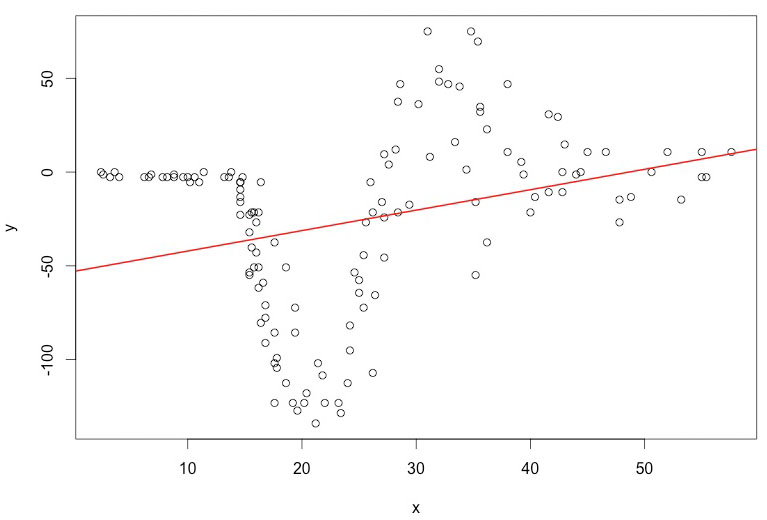
\includegraphics[width=14cm]{figure/mcyclelm}
\par\end{centering}

\caption{摩托车数据及其线性拟合图\label{fig:=006469=006258=008F66=006570=00636E=0053CA=005176=007EBF=006027=0062DF=005408=0056FE}}
\end{figure}


\begin{figure}[H]
\begin{centering}
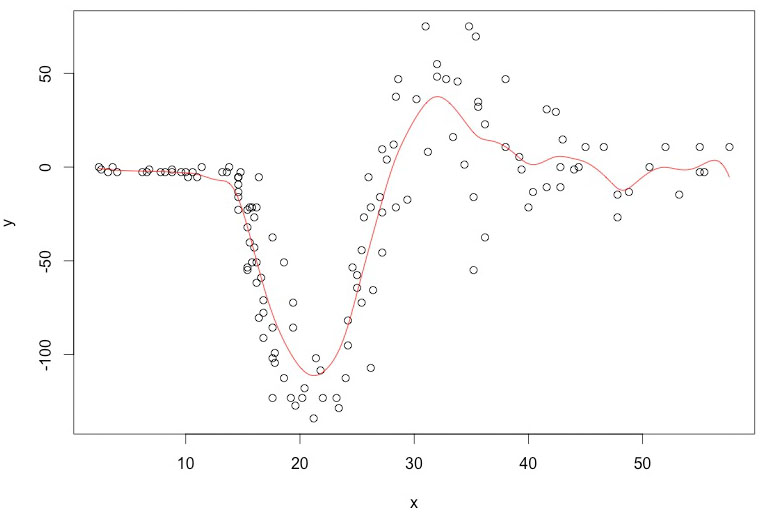
\includegraphics[width=14cm]{figure/mcycleloc}
\par\end{centering}

\caption{摩托车数据的非参数回归拟合图\label{fig:=006469=006258=008F66=006570=00636E=007684=00975E=0053C2=006570=0056DE=005F52=0062DF=005408=0056FE}}
\end{figure}


计算得到线性回归的拟合结果见图\ref{fig:=006469=006258=008F66=006570=00636E=0053CA=005176=007EBF=006027=0062DF=005408=0056FE},非参数回归见图\ref{fig:=006469=006258=008F66=006570=00636E=007684=00975E=0053C2=006570=0056DE=005F52=0062DF=005408=0056FE}。从这些图中我们可以清楚地看到,$Y_{i}$与$X_{i}$的关系是非线性关系,$ $给定已知的线性函数,拟合效果很差;即使使用其他已知的非线性函数,$Y_{i}$与$X_{i}$的拟合效果也显然不能令人满意。而在图\ref{fig:=006469=006258=008F66=006570=00636E=007684=00975E=0053C2=006570=0056DE=005F52=0062DF=005408=0056FE}中的非参数拟合图中我们可以看到非参数回归有很好的拟合效果,可以真实反映$Y_{i}$与$X_{i}$的实际关系(在不同的核函数和窗宽的选择下,拟合效果也有一定的差异)。$ $

\newpage{}
\bibliographystyle{XMU}
\setlength{\bibsep}{0.5ex}  %参考文献行距 
\phantomsection\addcontentsline{toc}{chapter}{参考文献}
%\addcontentsline{toc}{chapter}{参考文献}      % 参考文献加入到中文目录
\addcontentsline{toe}{chapter}{\bfseries  References} % 参考文献加入到英文目录
%\addtolength{\bibsep}{-0.8em}
\nocite{*}  %若将此命令屏蔽掉,则未引用的文献不会出现在文后的参考文献列表中。

\bibliography{Paper}




\end{document}
